% LINGI2251
% Development methods
\documentclass[11pt, a4paper]{article}
\usepackage[utf8]{inputenc}
\usepackage[UKenglish]{babel}
\usepackage{graphicx}				% Use pdf, png, jpg, or eps§ with pdflatex; use eps in DVI mode
\usepackage{xcolor}
\usepackage{listings}
\usepackage{hyperref}
\usepackage{array}
\usepackage{longtable}
\usepackage{multirow}
\usepackage[babel=true]{csquotes}


\usepackage[T1]{fontenc}

\lstset{%
	basicstyle=\ttfamily\footnotesize,
	commentstyle=\color{green!90!black},
	frame=single,
	keywordstyle=\bfseries\color{blue},
	language=python,
	numberstyle=\color{gray},
%	tabsize=2,
}


\hypersetup{%
	colorlinks=true,
	linkcolor=blue,
	urlcolor=blue
}


\newcommand{\tbf}[1]{\textbf{#1}}
\newcommand{\tit}[1]{\textit{#1}}

\newcommand{\data}[1]{\textit{#1}}
\newcommand{\state}[1]{\textsf{#1}}



\def\blurb{\textsc{Université catholique de Louvain\\
  École polytechnique de Louvain\\
  Pôle d'ingénierie informatique}}
\def\clap#1{\hbox to 0pt{\hss #1\hss}}%
\def\ligne#1{%
  \hbox to \hsize{%
    \vbox{\centering #1}}}%
\def\haut#1#2#3{%
  \hbox to \hsize{%
    \rlap{\vtop{\raggedright #1}}%
    \hss
    \clap{\vbox{\vfill\centering #2\vfill}}%
    \hss
    \llap{\vtop{\raggedleft #3}}}}%
\begin{document}

\begin{titlepage}
\thispagestyle{empty}\vbox to 1\vsize{%
  \vss
  \vbox to 1\vsize{%
    \haut{\raisebox{-2mm}{
\includegraphics[width=2.5cm]{logo_epl.jpg}}}{\blurb}{\raisebox{-5mm}{
\includegraphics[scale=0.20]{ingi_logo}}}
    \vfill
    \ligne{\Huge \textbf{\textsc{LINGI2251}}}
     \vspace{5mm}
    \ligne{\huge \textbf{\textsc{Development methods}}}
     \vspace{15mm}
    \ligne{\Large \textbf{\textsc{Assignment 1: The Gas Station Control System}}}
    \vspace{5mm}
    \ligne{\large{\textsc{March 23, 2015}}}
    \vfill
    \vspace{5mm}
    \ligne{%
         \textsc{Professor\\Charles Pecheur}
      }
      \vspace{10mm}
    }%
    \ligne{%
         \textsc{Michael Heraly\\Thibault Gerondal}
      }
      \vspace{5mm}
  \vss
  }
\end{titlepage}



\newpage


\section{Requirement issues}

\begin{itemize}

\item In the requirements, the term \textit{GSCS} is used a lot of time. We don't know if this term refers to a kind of interface or if it refers to the whole system. We'll assume that it refers to the whole system and that the cashier interface is responsible of saving all informations (does include a database).

\item There is no information that indicates how the cashier knows the price that the customer has to pay at the pump. We will therefore assume that the cashier is able to have an overview of all pumps (i.e. pumps send their states and informations to the cashier's interface).

\item We'll assume that the cashier's interface does include a credit card reader. This could be used by the customer to pay a monthly bill, since the requirement tells that \enquote{customers can always pay via cash or credit card}.

\item What are the steps to create a monthly billing account number ? We'll assume that the customer has to ask the cashier for creating a monthly billing account.

\item ``the paper credit card receipt will be photocopied and stored with the rest of the year’s receipts''. This requirement is ambiguous. This action has to be managed by the cashier. We can think of being able to save the scan of the credit card receipt in the database of the system via the cashier's interface.

\end{itemize}



\newpage
\section{Interfaces}

\subsection{Gas pump}

\begin{itemize}
\item Input :
		\begin{itemize}
		\item The trigger is pressed.
		\end{itemize}

\item Output :
		\begin{itemize}
		\item \data{Gallons} [positive float] : Number of gallons purchased. 
    \item \data{Dollars} [positive float; max 999,99] : Dollar amount of the purchase.
		\end{itemize}
\end{itemize}


\bigskip

\subsection{Gas pump interface}

\begin{itemize}
\item Input :
		\begin{itemize}
    \item \data{Gallons} [positive float] : Number of gallons purchased (from the Gas pump).
    \item \data{Dollars} [positive float, max 999,99] : Dollar amount of the purchase (from the Gas pump).
    \item \data{Payment Token} [integer representing a {valid, invalid} payment] : Token giving information about the payment (from the Credit Card System).
    \item \data{Reset Token} [integer representing a reset operation] : When the token is received, the pump is reset.
    \item \data{User input} [User choices] : The user can communicate his choice of payment.
    \end{itemize}

\item Output :
		\begin{itemize}
		\item \data{User output} [Strings] : Messages on the screen to guide the user through steps.
    \item \data{Gallons} [positive float] : Number of gallons purchased (to the cashier's interface).
    \item \data{Dollars} [positive float, max 999,99] : Dollar amount of the purchase (to the cashier's interface and to the card reader system).
		\end{itemize}
\end{itemize}



\newpage
\subsection{Credit card reader}

\begin{itemize}
\item Input :
		\begin{itemize}
		\item \data{Credit card number} : credit card number read.
		\end{itemize}

\item Output :
		\begin{itemize}
		\item \data{Credit card number} : send the credit car number to the gas pump interface.
		\item \data{Invalid token} : send an invalid token to the gas pump interface if the credit card number cannot be read correctly.
		\end{itemize}
\end{itemize}


\bigskip

\subsection{Credit card system}

\begin{itemize}
\item Input :
		\begin{itemize}
		\item \data{credit card number} : receive the credit card number from the gas pump interface.
		\item \data{purchase amount} : receive the purchase amount from the gas pump interface.
		\end{itemize}
\item Output :
    \begin{itemize}
    \item \data{Validation} : Send a validation token or an error token.
    \end{itemize}

\end{itemize}


\bigskip

\subsection{Cashier}

\begin{itemize}
\item Input :
		\begin{itemize}
		\item \data{cash} [positive float] : receive cash payments from customers.
		\end{itemize}

\item Output :
		\begin{itemize}
		\item \data{change} [positive float] : give money as change for the payment.
		\item \data{payment complete} : indicate that the payment is complete to the cashier's interface.
		\end{itemize}
\end{itemize}



\newpage
\subsection{Cashier's interface}

\begin{itemize}
\item Input :
		\begin{itemize}
		\item \data{type of payment} : the cashier indicates whether : 
					\begin{itemize}
					\item the payment has to be added to a monthly bill.
					\item the payment is done by credit card.
					\end{itemize}
		\item \data{billing account number} : the cashier enters the billing account number of the customer if the payment is to be made by monthly bill.
		\item \data{credit card account number} : the cashier enters the credit card account number if the customer pays by credit card.
		\item \data{payment complete} : the cashier indicates that the payment is complete.
		\end{itemize}

\item Output :
		\begin{itemize}
		\item \data{display purchase prices} : display the purchase prices.
		\item \data{display error messages} : display an error messages (e.g. if the billing account number entered is invalid).
    \item \data{Reset Token} [integer representing a reset operation] : when the token is sent to a pump, the pump is reset.
    \item Save every purchase in a database.
		\end{itemize}
\end{itemize}


\bigskip

\section{State of the system}

The GSCS stores the following data :
\begin{itemize}
\item Related to the gas station :
		\begin{itemize}
		\item \data{gallons purchased}
		\item \data{purchase amount}
		\end{itemize}

\item Related to the customers :
		\begin{itemize}
		\item \data{Personal informations} : name, address, phone number, billing account number.
		\item \data{Purchase informations} : how many gallons, the purchase amount, and the date.
		\item \data{Purchase status} : does the customer have a due amount, type of payment, date of the purchase, date of the payment.
		\end{itemize}
\end{itemize}


\newpage
\section{Data-flow diagram}

Typically, the customer pumps some gas. He then chooses the payment method from the gas pump interface. According to his choice, he ends up paying or giving his billing number to the cashier.

\begin{center}
\centerline{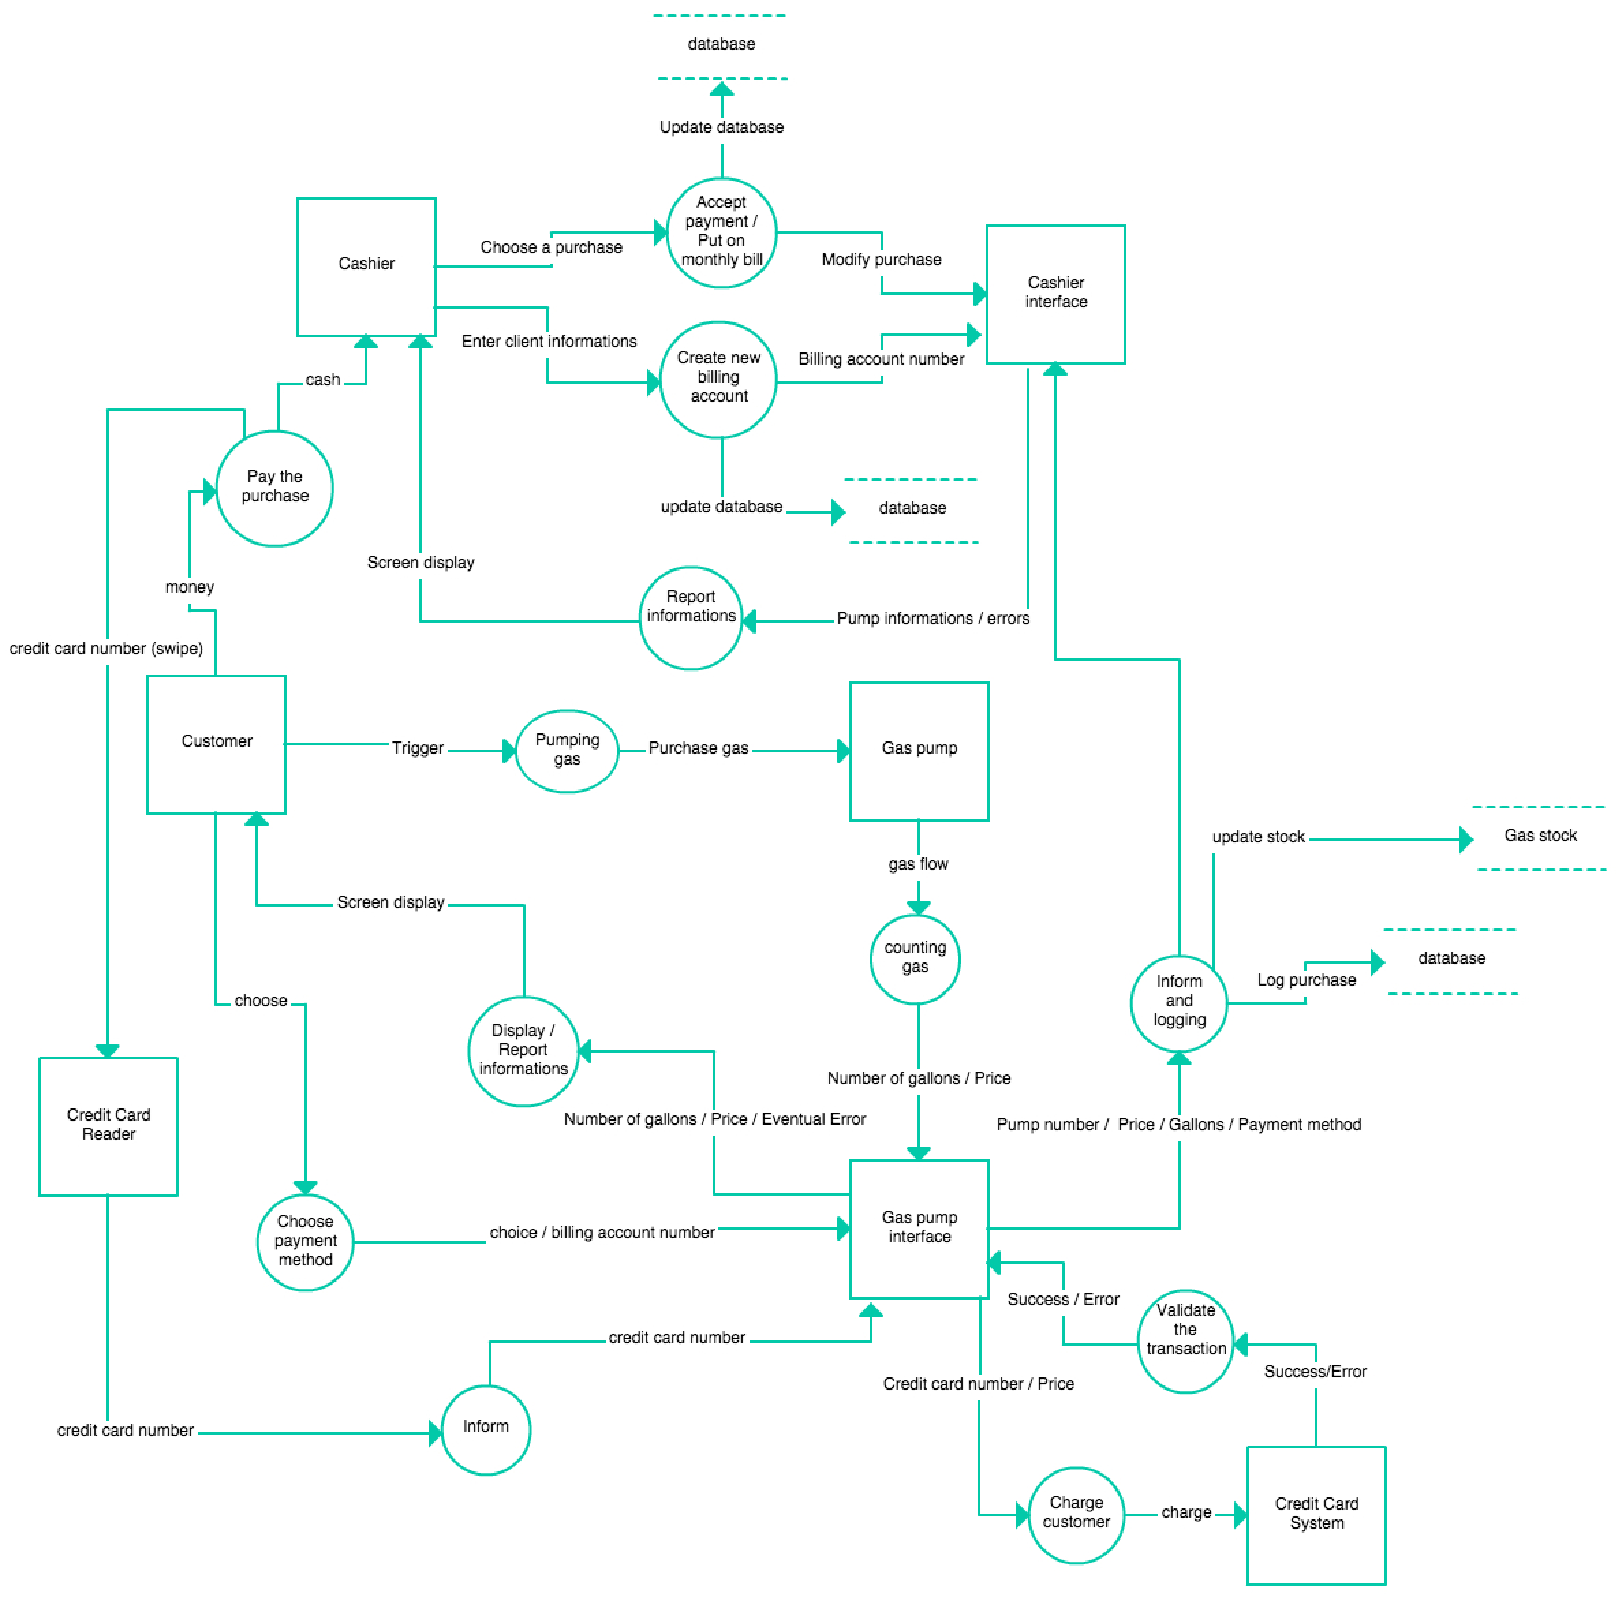
\includegraphics[width=1.4\textwidth]{dataflow_diagram.pdf}}
\end{center}

\section{Class diagram}

\begin{center}
\centerline{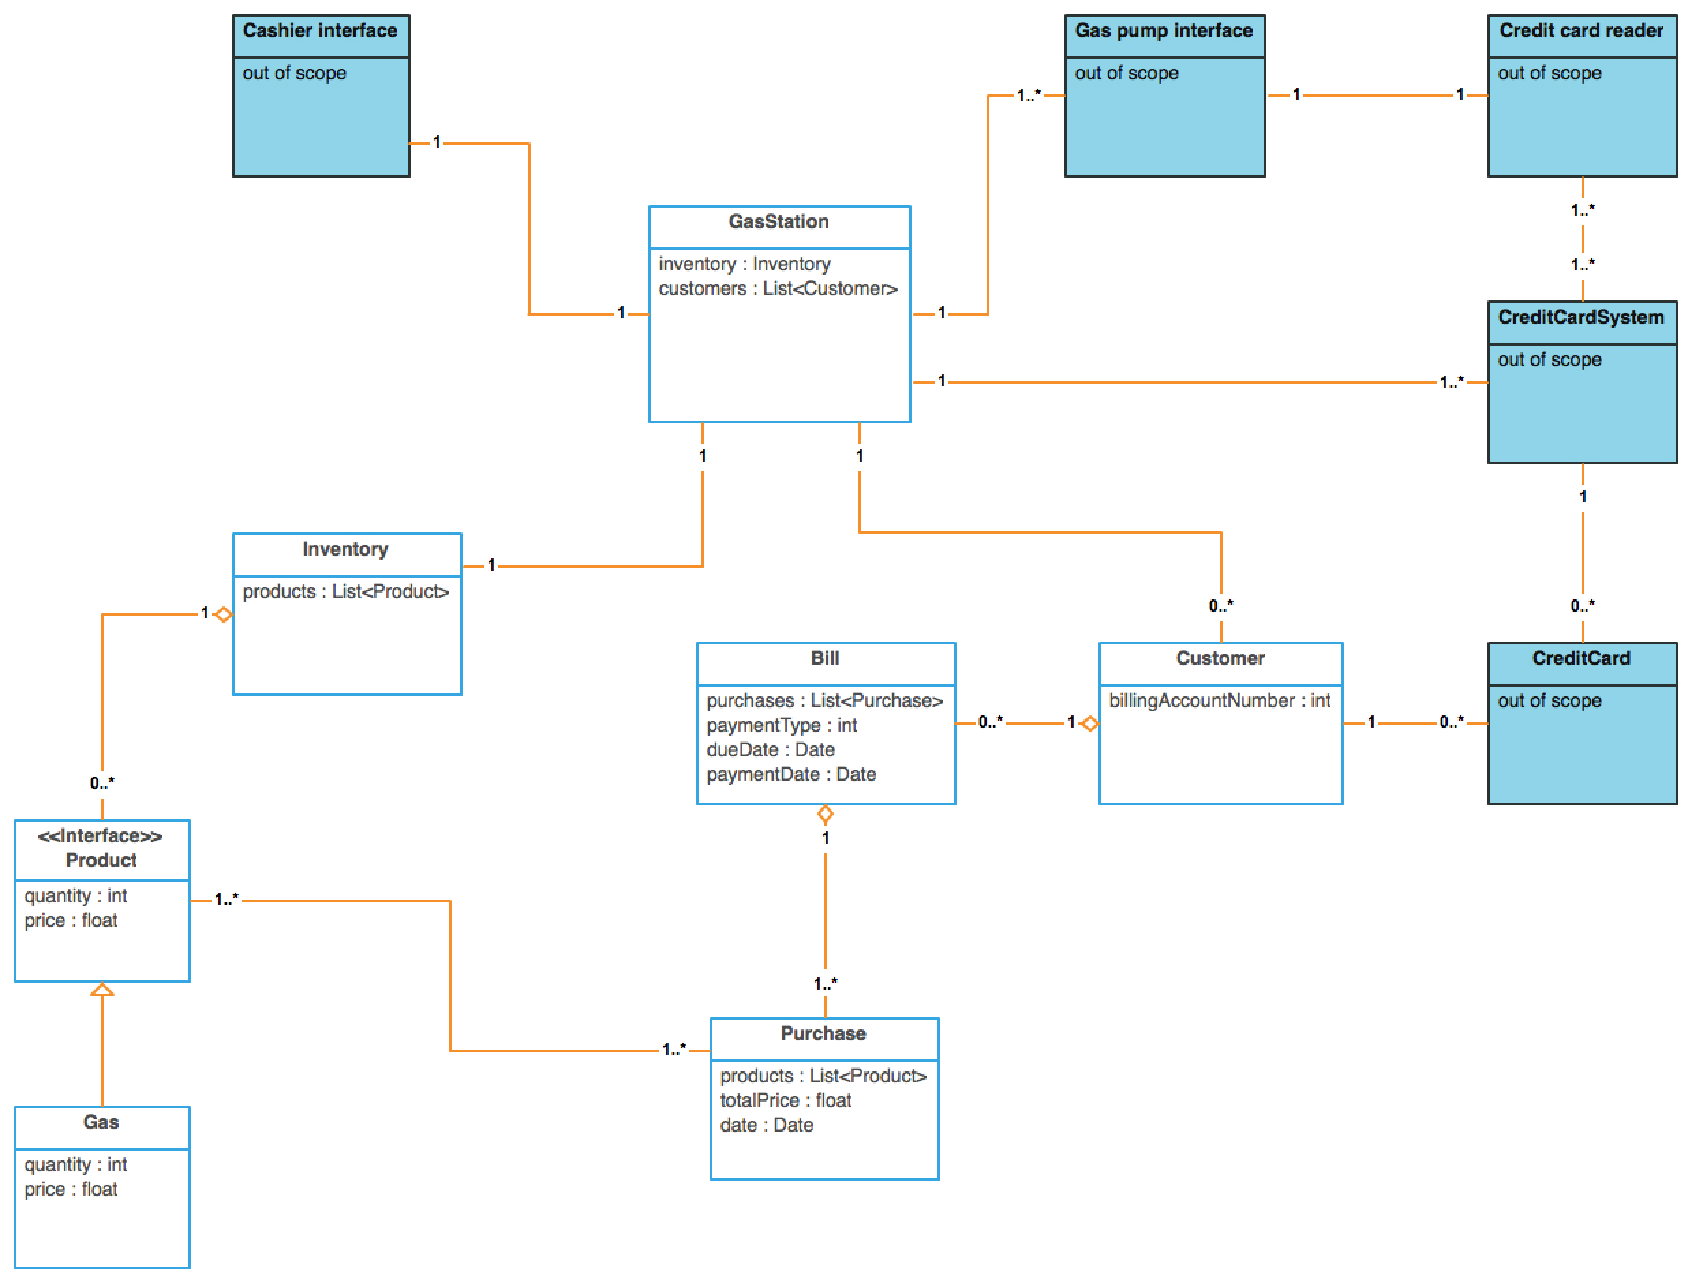
\includegraphics[width=1.3\textwidth]{Class_diagram.pdf}}
\end{center}


\section{Sequence diagrams}

\subsection{A customer successfully purchases gas and charges it on a monthly bill}


\begin{center}
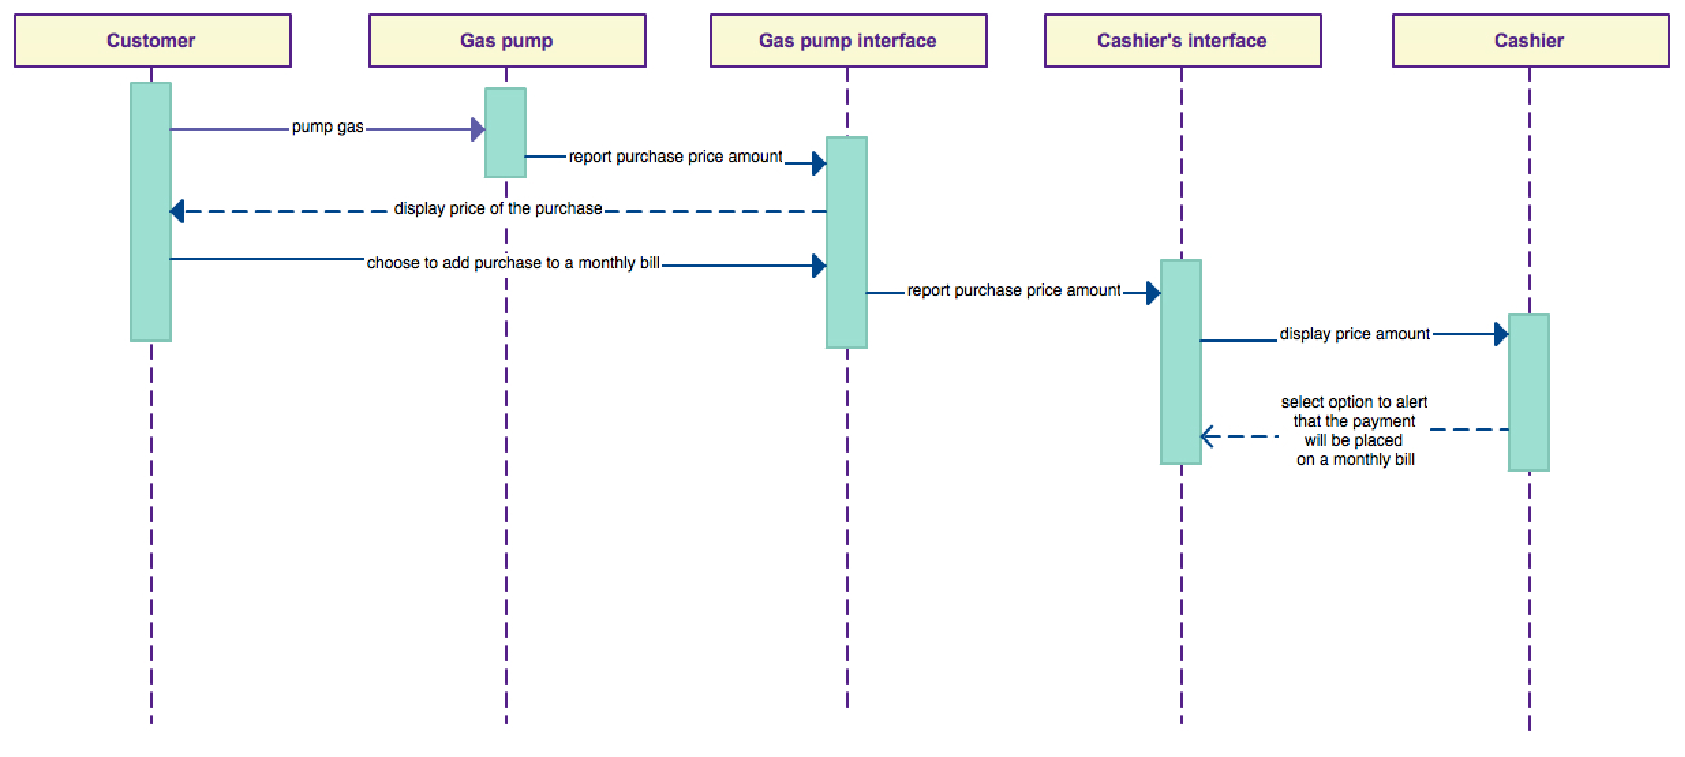
\includegraphics[width=17cm, angle=90]{SequenceDiagram_1_monthly_bill.pdf}
\end{center}


\subsection{A customer purchases gas and attempts to pay by credit card but his card is refused. He then pays by cash to the cashier}

\begin{center}
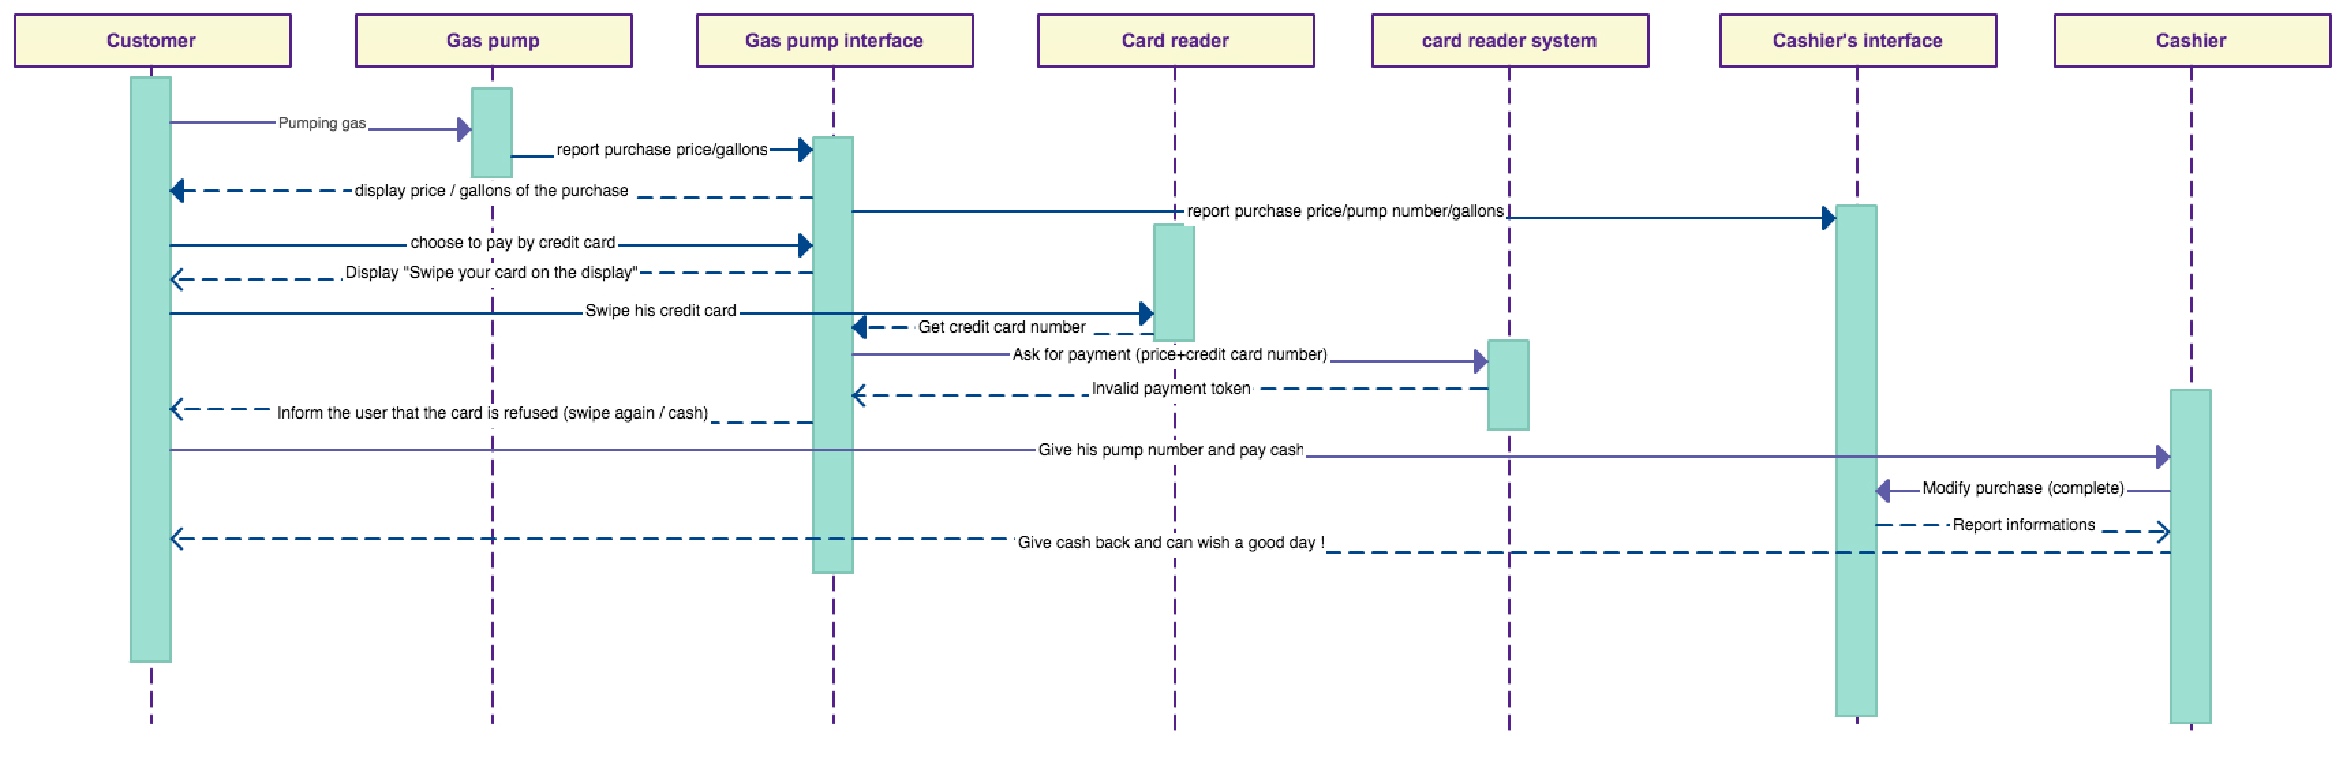
\includegraphics[width=17cm, height=8cm, angle=90]{credicash.pdf}
\end{center}

\newpage


\subsection{The cashier successfully processes a monthly payment by credit card}

\begin{center}
%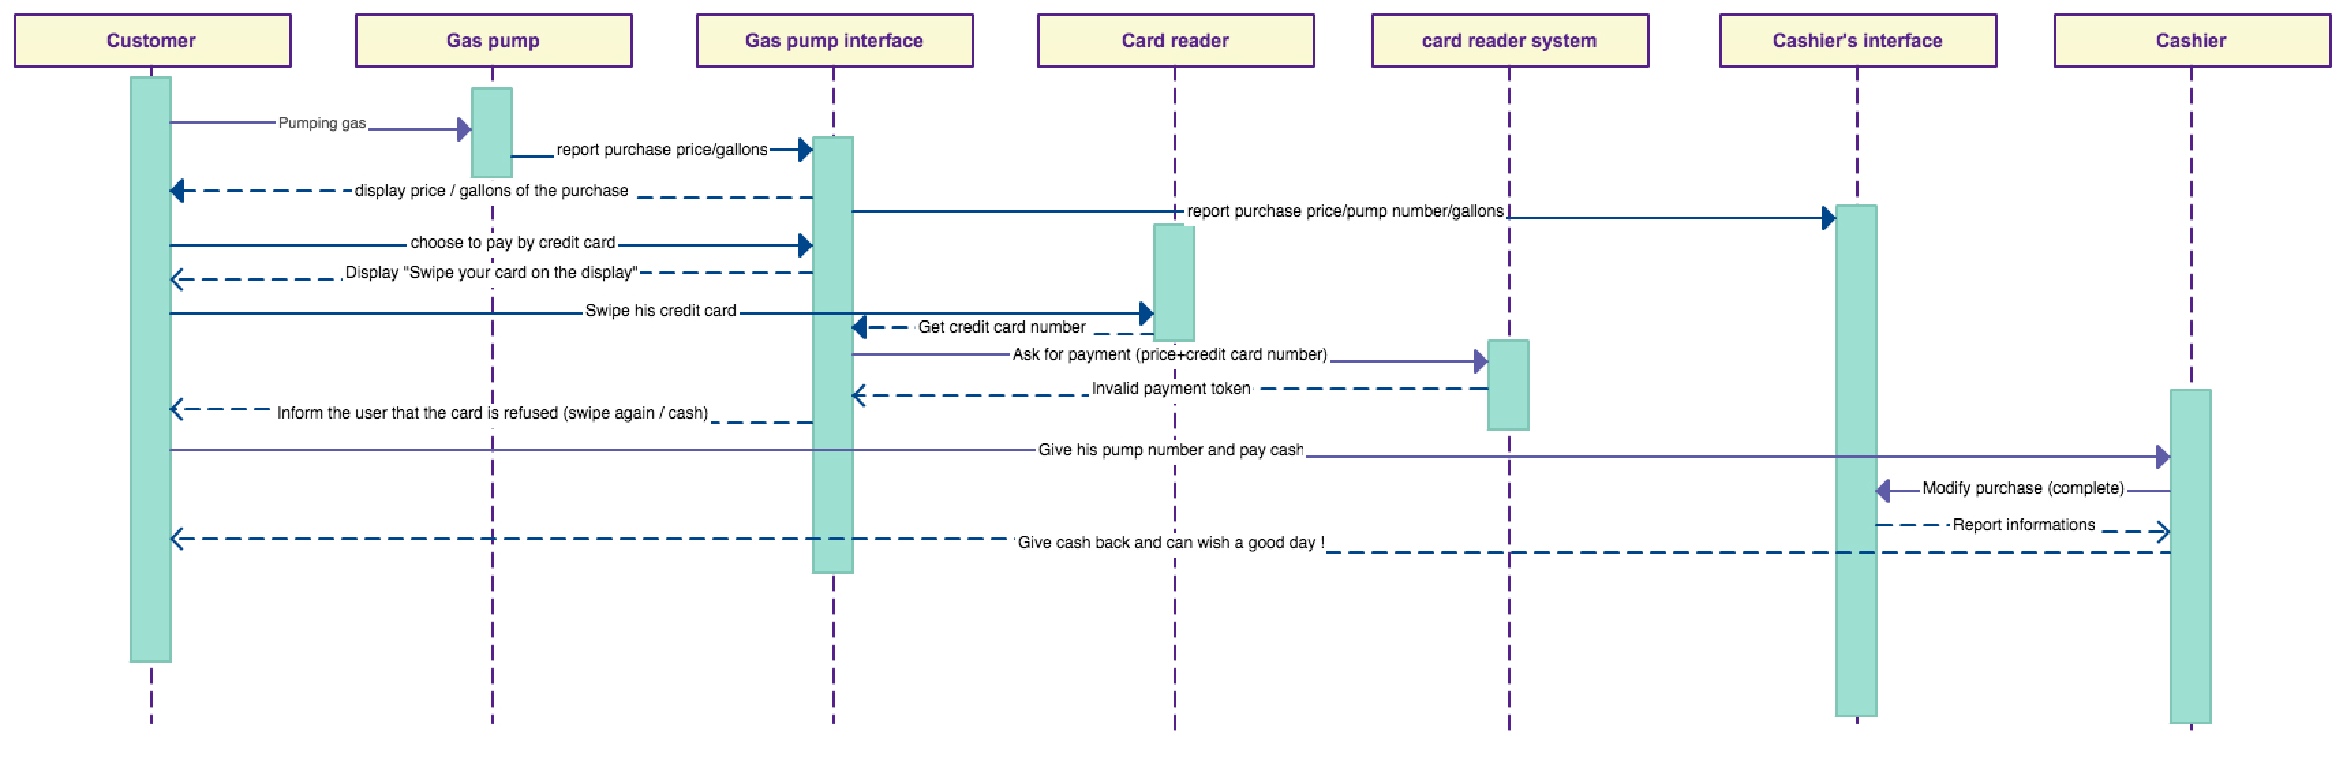
\includegraphics[width=17cm, height=8cm, angle=90]{credicash.pdf}
\end{center}


\newpage

\section{State diagrams}

\subsection{Gas Pump Interface}

\begin{center}
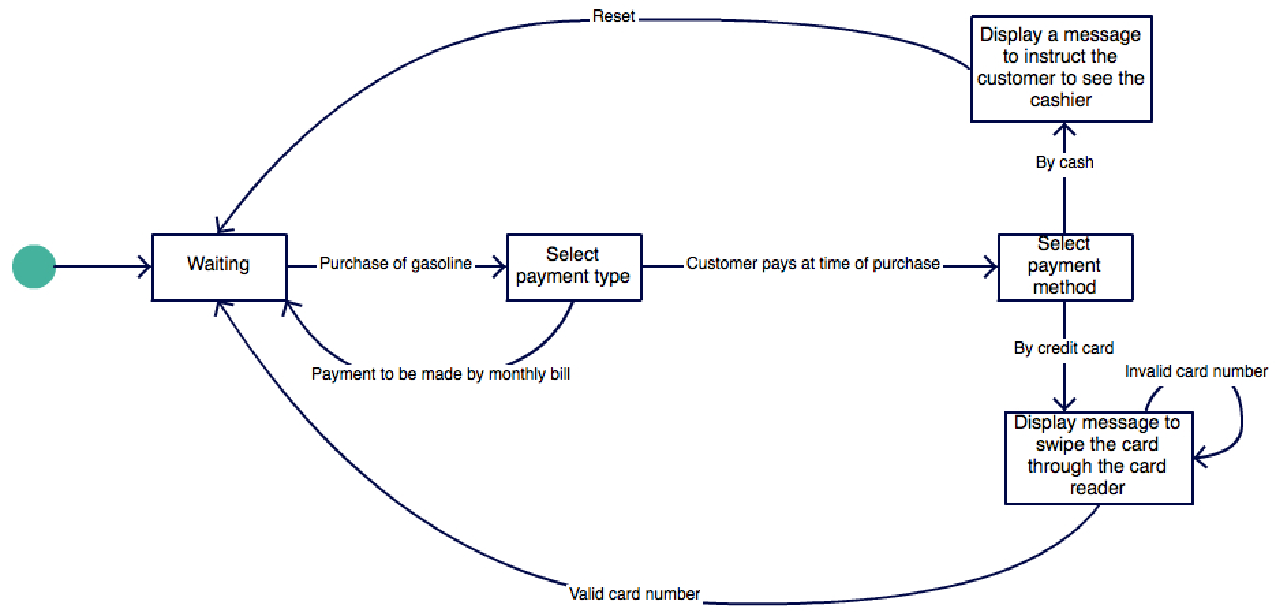
\includegraphics[width=\textwidth]{GasPumpInterface_diagram.pdf}
\end{center}


\subsubsection*{Description}

The start state of the Gas pump interface (GPI) is \state{Waiting}.
After the customer has used the pump to purchase gasoline, the GPI displays a menu for the customer to select the payment type.
If the payment is done by monthly bill, the GPI goes back to \state{Waiting} state.
If the customer choose to pay by credit card and that the credit card number is valid, it is sent to the credit card system and the GPI goes back to \state{Waiting} state.


\medskip

\subsection{Cashier's interface}

\begin{center}
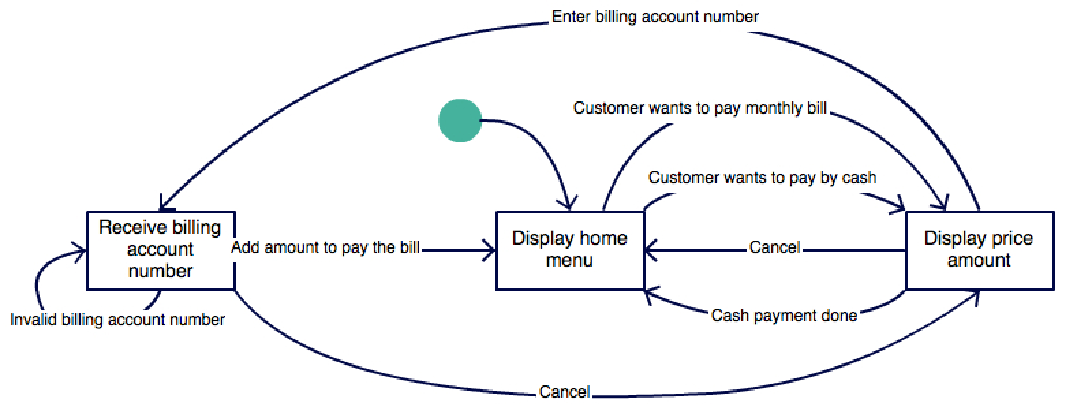
\includegraphics[width=\textwidth]{CashierInterface_diagram.pdf}
\end{center}

\subsubsection*{Description}

The start state of the Cashier's interface (CI) is \state{Display home menu}.
If the customer wants to pay a monthly bill, the cashier has to enter the billing account number.


\end{document}
